\documentclass[main.tex]{subfiles}
\begin{document}
\subsection{The waving of hands}
This section will informally give a basic idea for all concepts used throughout the text
with the sole purpose to give some intuition about the project end-to-end.

Our goal is to have our user write a query like this:
\begin{center}
    \code{pharmacies near parking spaces in Berlin}
\end{center}
And get such circles on a map as those shown in \cref{fig:circles}.

\cfigure{
    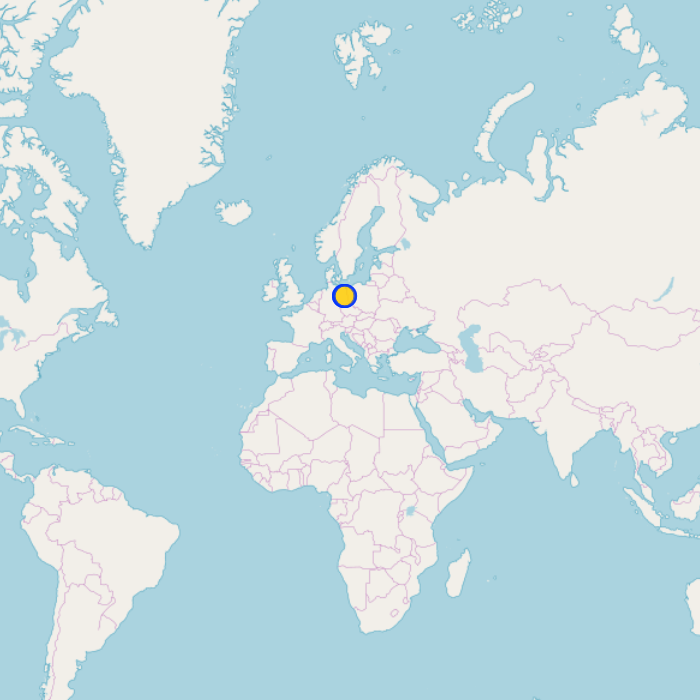
\includegraphics[width=0.32\textwidth]{map/world.png}
    \hfill
    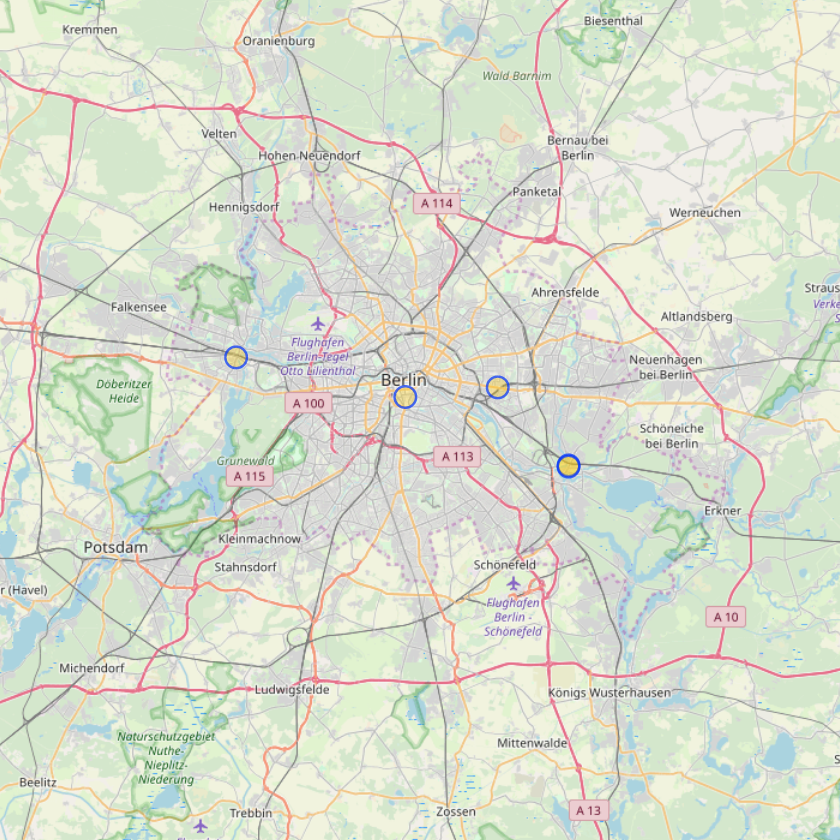
\includegraphics[width=0.32\textwidth]{map/berlin.png}
    \hfill
    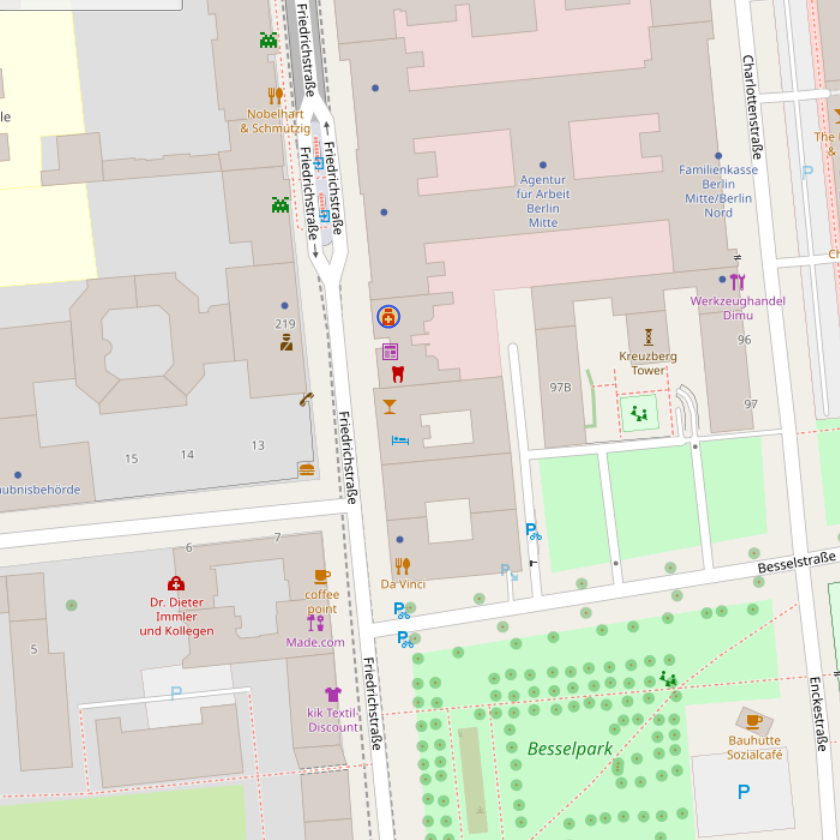
\includegraphics[width=0.32\textwidth]{map/pharmacy.png}
    \caption{Wanted result for query ``pharmacies near parking spaces in Berlin''}
    \label{fig:circles}
}

To do this, we will first construct a Combinatory Categorial Grammar which parses
such queries. The central idea of CCG is that each word (or terminal) is assigned
a set of
\emph{categories}, which work the same way as types work in programming
languages\footnote{Especially curried programming languages like Haskell}.
Semantically, each word returns something and may take other things as arguments.

Here, our basic type will be called $GSet$ and will mean "a set of geographic
objects". Each basic type is also a category.

So, we can immediately assign the category of \code{pharmacies} and of
\code{Berlin} to be $GSet$ - they will have the semantics of ``the set of all
pharmacies'' and ``the singleton of the city of Berlin'' respectively:
\gramshort{
    \gramrow{pharmacies}{ GSet }{}
    \gramrow{Berlin}{ GSet }{}
}

Now, we want \code{parking spaces} to have a $GSet$ category and the semantics
of ``the set of all parking spaces''. One way to do this is to assign a special
category $Spaces$ to the word \code{spaces}, and make \code{parking} take
$Spaces$ as an argument on the right and returns $GSet$. We will denote this
``argument on the right'' construction by a forward slash:
\gramshort{
    \gramrow{parking}{ GSet \rc Spaces }{}
    \gramrow{spaces}{Spaces}{}
}
Coincidentally, arguments on the left will be denoted by a backward slash.

Now, we need to assign a category to the word \code{in}. We want to parse
the construction ``something in something'', thus we want to take one $GSet$
on the left and one $GSet$ on the right, and return another $GSet$:
\gramshort{
    \gramrow{in}{ (GSet \lc GSet) \rc GSet }{}
}
This means that \code{in} will take a $GSet$ on the right and produce something
which takes another $GSet$ on the left and returns the final $GSet$.
In our case, \code{in Berlin} takes something of type $GSet$ on the left and
returns a $GSet$.
An alternative category that would also work is the following:
\gramshort{
    \gramrow{in}{ (GSet \rc GSet) \lc GSet }{}
}
In this case, \code{in Berlin} makes no sense, but \code{parking spaces in}
will return something that will gladly take \code{Berlin} on the right and
produce a $GSet$.

The syntax of ``near'' is similar to the syntax of ``in'', so we will assign
the same category. Finally, we get this simple grammar:
\gramshort{
    \gramrow{pharmacies}{ GSet }{}
    \gramrow{Berlin}{ GSet }{}
    \gramrow{parking}{ GSet \rc Spaces }{}
    \gramrow{spaces}{Spaces}{}
    \gramrow{in}{ (GSet \lc GSet) \rc GSet }{}
    \gramrow{near}{ (GSet \lc GSet) \rc GSet }{}
}
Which will parse our query. The most convenient way to illustrate such parses
is by means of a \emph{derivation tree}:
\centree{.{$GSet$}
    [ .{$GSet$}
        [ .{$GSet$} [ .{$pharmacies$} ] ]
        \edge[very thick];
        [ .{$GSet \lc GSet$}
            \edge[very thick];
            [ .{$(GSet \lc GSet) \rc GSet$} [ .{$near$} ] ]
            [ .{$GSet$}
                \edge[very thick];
                [ .{$GSet \rc Spaces$} [ .{$parking$} ] ]
                [ .{$Spaces$} [ .{$spaces$} ] ]
            ]
        ]
    ]
    \edge[very thick];
    [ .{$GSet \lc GSet$}
        \edge[very thick];
        [ .{$(GSet \lc GSet) \rc GSet$} [ .{$in$} ] ]
        [ .{$GSet$} [ .{$Berlin$} ] ]
    ]
}

Here, a thick line signifies the ``function'' while a thin line signifies the
``argument''.

We can see that this derivation tree simply takes the building blocks produced
by the words and combines them in pairs until we get a single result. This means
we have assumed that the semantics of the language are \emph{compositional} -
larger sentences have semantics that can be described by composing the semantics
of its constituent subsentences.

Now, if we replace each word in the derivation tree by a building block of another
target language, and assume that we have chosen blocks with the same semantics,
we will compose a sentence in the other language that has the same meaning!
Of course, those suppositions (the compositional nature of the language and
that we can chose terminals with the same semantics) are utterly naïve,
especially for natural languages. But, if we restrict ourselves to a limited
domain within the natural language and generate sentences in a formal language,
those assumptions might give us acceptable results.

Ideally, we want to generate the following Overpass query:
\begin{lstwrap}\begin{lstlisting}
( node["amenity" = "parking_space"]; ) -> .x1;
( area["name" = "Berlin"]; area["int_name" = "Berlin"]; area["name:en" = "Berlin"]; ) -> .x2;
( node(area.x2)(around.x1:100.0)["amenity" = "pharmacy"]; ) -> .x3;
.x3 out;
\end{lstlisting}\end{lstwrap}

Since the compositional nature in Overpass is hidden, instead of generating
it directly we will generate a query in a custom intermediate language we will
call Minipass. In Minipass, the same query will look like this:
\begin{lstwrap}\begin{lstlisting}
    and (and (amenity 'pharmacy') (near (amenity 'parking_space'))) (in (name 'Berlin'))
\end{lstlisting}\end{lstwrap}

We will now assign a Minipass term to each of the words in our example (denoted
after the \code{@} symbol):
\gramshort{
    \gramrow{pharmacies}{ GSet }{\text{\code{amenity 'pharmacy'}}}
    \gramrow{Berlin}{ GSet }{\text{\code{name 'Berlin'}}}
    \gramrow{parking}{ GSet \rc Spaces }{\text{\code{lambda x => amenity 'parking\_space'}}}
    \gramrow{spaces}{Spaces}{\text{\code{lambda x => x}}}
    \gramrow{in}{ (GSet \lc GSet) \rc GSet }{\text{\code{lambda x, y => and y (in x)}}}
    \gramrow{near}{ (GSet \lc GSet) \rc GSet }{\text{\code{lambda x, y => and y (near x)}}}
}

We can now see how the tree will compose these terms:
\autoscaledtree{.{\code{and (and (amenity 'pharmacy') (near (amenity 'parking_space'))) (in (name 'Berlin'))}}
    [ .{\code{and (amenity 'pharmacy') (near (amenity 'parking\_space'))}}
        [ .{\code{amenity 'pharmacy'}} [ .{$pharmacies$} ] ]
        \edge[very thick];
        [ .{\code{lambda y => and y (near (amenity 'parking\_space'))}}
            \edge[very thick];
            [ .{\code{lambda x, y => and y (near x)}} [ .{$near$} ] ]
            [ .{\code{amenity 'parking\_space'}}
                \edge[very thick];
                [ .{\code{lambda x => amenity 'parking\_space'}} [ .{$parking$} ] ]
                [ .{\code{lambda x => x}} [ .{$spaces$} ] ]
            ]
        ]
    ]
    \edge[very thick];
    [ .{\code{lambda y => and y (in (name 'Berlin'))}}
        \edge[very thick];
        [ .{\code{lambda x, y => and y (in x)}} [ .{$in$} ] ]
        [ .{\code{name 'Berlin'}} [ .{$Berlin$} ] ]
    ]
}

Note that ``lambda'' expressions have been ``reduced'' in order to decrease
clutter. We will later formally explain their semantics and how to do that.

This produces the exact Minipass query we wanted. The grammar can now be extended
to cover many more types of queries.

The last thing we will do is create a translator from Minipass to Overpass
to complete the pipeline in \cref{fig:pipeline}.

\cfigure{
    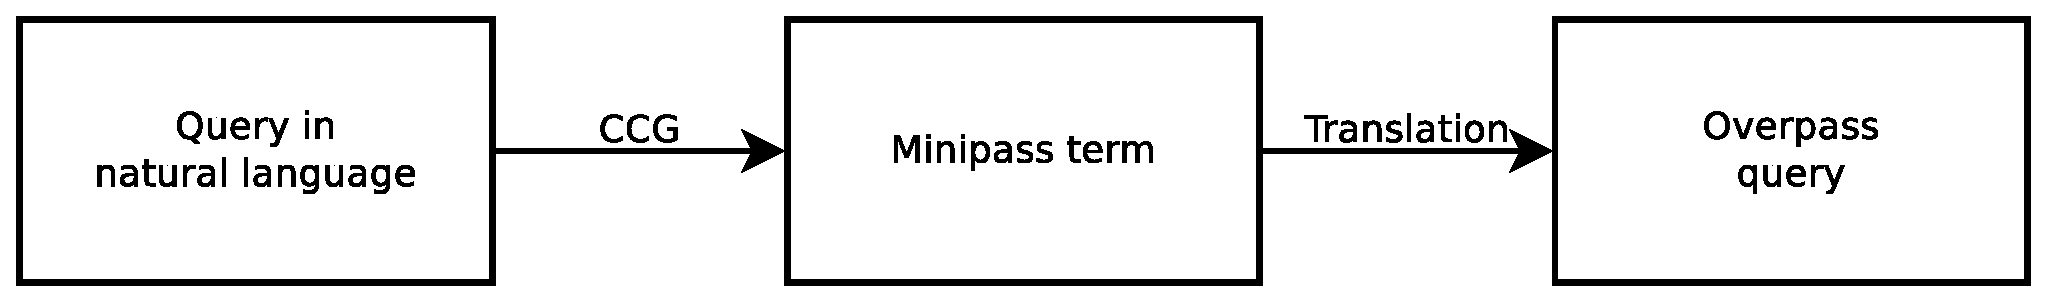
\includegraphics[width=0.8\textwidth]{pipeline.eps}
    \caption{General pipeline for a query}
    \label{fig:pipeline}
}
\end{document}
